\documentclass{article}

\usepackage[a4paper]{geometry}
\usepackage[ngerman]{babel}
\usepackage[utf8]{inputenc}
\usepackage[T1]{fontenc}
\usepackage{tabularx}
\usepackage{graphicx}

\graphicspath{ {./images/} }

\setlength{\tabcolsep}{1em}
\def\arraystretch{1.5}

\begin{document}

\begin{titlepage}
	\begin{flushleft}
		TH Brandenburg \\
		Online Studiengang Medieninformatik \\
		Fachbereich Informatik und Medien \\
		Datenbanken \\
		Prof. Dr.-Ing. Thomas Preuß
	\end{flushleft}

	\vfill

	\begin{center}
		\Large{Einsendeaufgabe 2: Relationales Modell}\\[0.5em]
		\large{Sommersemester 2021}\\[0.25em]
		\large{Abgabetermin 06.05.2021}
	\end{center}

	\vfill

	\begin{flushright}
		Maximilian Schulke \\
		Matrikel-Nr. 20215853
	\end{flushright}
\end{titlepage}

\newpage

\section{Vorgegebene Musterlösung}

\begin{figure}[h!]
	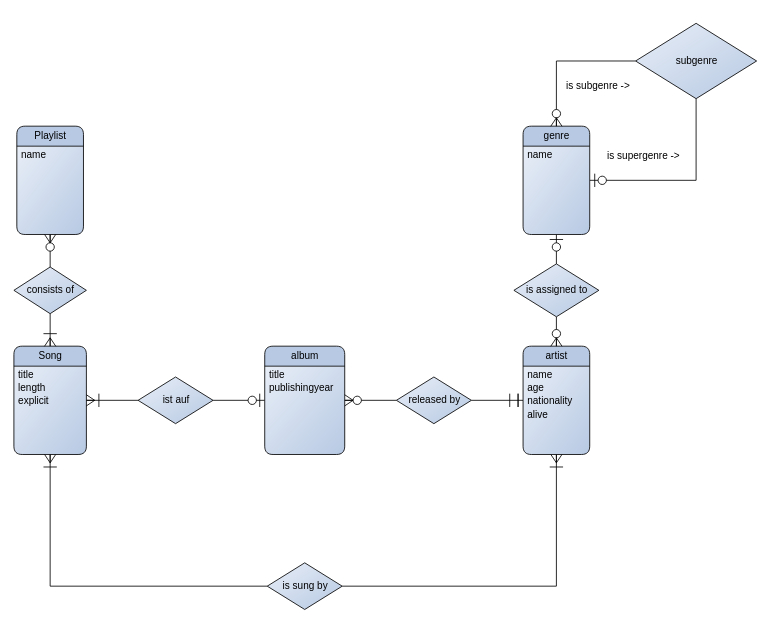
\includegraphics[width=\textwidth]{er.jpg}
	\centering
	\caption{Die im Moodle-Kurs vorgegebene Musterlösung}
\end{figure}

\newpage

\section{Relationales Modell}

\subsubsection*{Legende}

\begin{itemize}
	\item[] \underline{Primärschlüssel}
	\item[] \textit{Fremdschlüssel}
	\item[] \underline{\textit{Fremdschlüssel der Teil des Primärschlüssels ist}}
\end{itemize}

\subsubsection*{playlist}

\begin{tabularx}{4cm}{|X|X|}
	\hline
	\underline{id} & name \\
	\hline
\end{tabularx}

\subsubsection*{playlist\_consists\_of\_song}

\begin{tabularx}{6cm}{|X|X|}
	\hline
	\underline{\textit{playlist\_id}} & \underline{\textit{song\_id}} \\
	\hline
\end{tabularx}

\subsubsection*{song}

\begin{tabularx}{10cm}{|X|X|X|X|X|}
	\hline
	\underline{id} & title & length & explicit & \textit{album} \\
	\hline
\end{tabularx}

\subsubsection*{album}

\begin{tabularx}{9cm}{|X|X|m{3cm}|X|}
	\hline
	\underline{id} & title & publishingyear & \textit{artist} \\
	\hline
\end{tabularx}

\subsubsection*{artist}

\begin{tabularx}{13cm}{|X|X|X|m{3cm}|X|X|}
	\hline
	\underline{id} & name & age & nationality & alive & \textit{genre} \\
	\hline
\end{tabularx}

\subsubsection*{song\_sung\_by\_artist}

\begin{tabularx}{6cm}{|X|X|}
	\hline
	\underline{\textit{song\_id}} & \underline{\textit{artist\_id}} \\
	\hline
\end{tabularx}

\subsubsection*{genre}

\begin{tabularx}{7cm}{|X|X|m{3cm}|}
	\hline
	\underline{id} & name & \textit{supergenre} \\
	\hline
\end{tabularx}

\end{document}